\chapter[Special Surveys]{Special Surveys}
\def\chpname{specialsurveys}\label{chp:\chpname}

\noindent {\it
Knut Olsen, David Nidever, more to come
}

% Confirmed leads for LMC/SMC: Knut Olsen, David Nidever

% Confirmed leads for special surveys:

% --------------------------------------------------------------------

\section{Introduction}
\label{sec:specials:intro}

% Introduce, with a very broad brush, this chapter's science projects,
% and why it makes sense for them to be considered together.

The four main LSST science themes, as defined by the Science Book, drive the design of LSST's main Wide-Fast-Deep survey.  However, it has always been recognized that many important scientific projects, including some that are highly relevant to LSST's main science themes, are not well served by the areal coverage and/or cadence constraints placed on the WFD survey.  The LSST Project thus set aside a nominal 10\% of the observing time to serve what are collectively called ``special surveys''.  In addition, the LSST commissioning period may be available for use by special programs.  Projects that will certainly make use of this 10\% time not dedicated to the WFD survey include the Deep Drilling fields and Galactic Plane surveys described separately in this paper, as well as any survey wishing to observe at declinations below $-60^\circ$, such as the Magellanic Clouds.  These special programs heavily oversubscribe the nominal 10\% of time assigned to them.  It is of thus critical importance for these programs to define compelling science cases, clearly justify their observing requirements, and derive metrics to quantify the performance of a given schedule for the program.  An extra degree of freedom that these special surveys 


As mentioned previously, the Deep Drilling and Milky Way plane surveys are described separately in this paper.  In this section, we describe the goals of two special surveys designed to serve scientific goals related to the Magellanic Clouds.  Descriptions of other special surveys, including candidate commissioning programs, are welcome here.


% Add sections below, one science investigation per section, one
% section per file.
% --------------------------------------------------------------------

% ====================================================================

\chapter{The Magellanic Clouds}
\def\chpname{MCs}\label{chp:\chpname}

Chapter Editors:
\credit{dnidever},
\credit{knutago}

% \section*{Summary}
% \addcontentsline{toc}{section}{~~~~~~~~~Summary}
%
% Executive summary goes here, highlighting the primary conclusions from
% the chapter's science cases. This should be abstract length, no more:
% say, 200 words.

\section{Introduction}

The Magellanic Clouds have always had outsized importance for
astrophysics.  They are critical steps in the cosmological distance
ladder, they are a binary galaxy system with a unique interaction
history, and they are laboratories for studying all manner of
astrophysical phenomena.  They are often used as jumping-off points
for investigations of much larger scope and scale; examples are the
searches for extragalactic supernova prompted by the explosion of
SN1987A and the dark matter searches through the technique of
gravitational microlensing.  More than 17,000 papers in the NASA ADS
include the words ``Magellanic Clouds'' in their abstracts or as part
of their keywords, highlighting their importance for a wide variety of
astronomical studies.

An LSST survey that did not include coverage of the Magellanic Clouds
and their periphery would be tragically incomplete.  LSST has a unique
role to play in surveys of the Clouds.  First, its large $A\Omega$
will allow us to probe the thousands of square degrees that comprise
the extended periphery of the Magellanic Clouds with unprecedented
completeness and depth, allowing us to detect and map their extended
disks, stellar halos, and debris from interactions that we already
have strong evidence must exist.  Second, the ability of LSST
to map the entire main bodies in only a few pointings will allow us to
identify and classify their extensive variable source populations with
unprecedented time and areal coverage, discovering, for example,
extragalactic planets, rare variables and transients, and light echoes
from explosive events that occurred thousands of years ago (REFS).
Finally, the large number of observing opportunities that the LSST
10-year survey will provide will enable us to produce a static imaging
mosaic of the main bodies of the Clouds with extraordinary image
quality, an invaluable legacy product of LSST.

We have several important scientific questions:
\begin{enumerate}

\item What are the stellar and dark matter mass profiles of the
Magellanic Clouds?  To answer this we need to map their extended disks, halos, debris, and streams.  We can use
streams and RR Lyrae stars as probes of the 3D mass profile.

\item What is the satellite population of the Magellanic Clouds? The
discovery of dwarf satellites by the Dark Energy Survey and other
surveys hint at LSST's potential here.

\item What are the internal dynamics of the Magellanic Clouds?  Proper
motions from HST and from the ground have measured the bulk
motions of the Clouds and have, in combination with spectroscopy,
begun to unravel the three dimensional internal dynamics of the
Clouds.

\item How do exoplanet statistics in the Magellanic Clouds compare to
those in the Milky Way?  The calculations in the next section show that
LSST can measure transits of Jupiter-like planets, an intriguing
prospect given the Clouds' lower metallicity environment.

\item What are the variable star and transient population of the Clouds?
LSST will enable population studies, linking star formation and chemical
enrichment histories.

\item What can we learn about supernovae and other explosive events from
their light echoes?  Echoes can give view of such events unavailable by
any other means.

\end{enumerate}


These questions can be grouped into main overarching science themes:
\begin{enumerate}
\item {\bf Galaxy formation evolution}: The study of the formation and
evolution of the Large and Small Magellanic Clouds (LMC and SMC,
respectively), especially their interaction with each other and the
Milky Way. The Magellanic Clouds (MCs) are a unique local laboratory
for studying the formation and evolution of dwarf galaxies in
exquisite detail.  LSST's large FOV will be able to map out the
three-dimensional structure, metallicity and kinematics in great
detail.
\item {\bf Stellar astrophysics \& Exoplanets}:  The MCs have been
used for decades to study stellar astrophysics, microlensing and other
processes.  The fact that the objects are effectively all at a single
known distance makes it much easier to study them than in, for
example, the Milky Way.  LSST will extend these studies to fainter
magnitudes, higher cadence, and larger area.
\end{enumerate}

Many different types of objects and measurements with their own
cadence ``requirements'' will fall into these two broad categories
(with some overlap).
% These will be outlined in the next section.
A very important aspect of the ``galaxy evolution'' science theme is
not just the cadence but also the sky coverage of the Magellanic
Clouds ``mini-survey.''  A common misunderstanding is that the MCs
only cover a few degrees on the sky.  That is, however, just the
central regions of the MCs akin to the thinking of the Milky Way as
the just the bulge.  The full galaxies are actually much larger with
LMC stars detected at $\sim$21$^{\circ}$ ($\sim$18 kpc) and SMC stars
at $\sim$10$^{\circ}$ ($\sim$11 kpc) from their respective centers.
The extended stellar debris from their interaction likely extends to
even larger distances.  Therefore, to get a complete picture of the
complex structure of the MCs will require a mini-survey that covers
$\sim$2000 deg$^2$.
% At this point, it not entirely clear how to
% include this into the metrics.
Note, that for the second science case
this is not as much of an issue since the large majority of the
relevant objects will be located in the high-density, central regions
of the MCs.

Our investigation of how the LSST observing strategy will affect the
science outline here is still in its infancy. Some of the disgnostic and
figure of merit metrics developed elsewhere in this paper may be useful
for assessing the Magellanic Cloud science cases as well. In the
meantime we present below two science cases in the early stages of development that show some of the promise LSST shows in this area.

% static science vs. variables
% cadence vs. areal coverage
%  -want to cover whole SCP area to some necessary depth
%  -cadence for time-variable objects in full area or portion
%    what's the minimal # of visits (with decent phase coverage) to do this?  ask Kathy
%    Paula Szkody white paper on doing the full MCs for variables, linked to old MC cadence page
%   maybe a separate metric for spatial structure
%   -variabes:  ability to recover period, classify,


% --------------------------------------------------------------------
%
% \new{Below is a generic list of things we want to measure in the
% Magellanic Clouds.}
% % These will need to be divided among a small set of
% % science sections, each describing a focused science project that has a
% % figure of merit, that is a function of various diagnostic metrics. The
% % final version of the chapter tex file probably will not contain this
% % list.
%
% \begin{enumerate}
%
% \item Deep Color Magnitude Diagrams
% %  -Deep CMDs, just a matter of number of visits
% %  -do the full SMASH (and relevant DES area) with full spatial coverage, at least to SMASH depths, smaller
% %  number of epochs, ~5 sigma at gri~25
% % Knut thoughts: I think we want to make sure that we get 1 mag below old turnoff out to 100 kpc in ugriz with 10sigma precision, i.e. ugriz~25
%
%
% \item Proper Motions
% %-Proper Motions, cadence not as much of an issue, just more epochs
% %  bulk proper motion
% %  LMC spiral motion, streaming motions
% %  internal velocity dispersion
%
%
% %\item Parallaxes
% %-Parallaxes, also mostly a function of nubmer of epochs
% %  bulk distances
% %  internal distance spread
% %  -probably not get parallaxes at MC distances, but could do foreground rejection
%
% \item Variable stars
%
% %-Variables, RR Lyrae, Cepheids might be too bright, dwarf cepheids/scuti good, many more of them.
% %   especially good for getting the 3D structure (out to large distances) of the MCs
% %   -eclipsing binaries (get very accurate distances, see OGLE paper), pulsating WDs, CVs, T Tauri stars
% % novae, supernovae  in Paula's white paper
%
% % use MCs are a way to get templates for variable sources that LSST will detect all over the sky
% % look at variable group metrics
%
%
% \item Transients
% %-Transients, dwarf novae
% % Mike Lund will work on some text for this.  Also did work on cadence considerations
% % for detecting periodic objects in general (periodogram purity function).
%
% \item Transiting Exoplanets
% % -Transiting planets, Mike Lund
% % -need deep drilling to have any hope of finding them
% % -best between ~0.8-1.6 Msun to detect exoplanets, not too faint
% % -can't get ingress/egress but can detect the dip and periodicity
% %   that's enough to characterize
% % -challenging to do follow-up because they are quite faint and too many (?)
% % -cadence?  cover all timescales properly
% % -what's the expected period distribution
%
% % See Lund et al.\ (2015) and the exoplanet discussion in previous part
% % of this paper.
%
% % PASP
%
% %\item Astrometric binaries
% %-Astrometric binaries
%
% \item Light-echoes
% % it's a surface-brightness issue, can see fainter things with LSST than MOSAIC/DECAM
% % could trace out lightcurve if more epochs
%
% \item Gyrochronology
% %-Gychronology, need to get periods of the dwarfs, gives age information
% %  -gyro periods are ~10 days at 1 Gyr and ~30 days at 10 Gyr
%
% \item Interstellar scintillation
% % run in movie mode for 1-2 nights to find missing molecular gas (H2)
% % https://github.com/LSSTScienceCollaborations/ObservingStrategy/issues/68
%
% % Legacy survey
% % use the best seeing to get great data on the MC main bodies
%
% %\item Astroseismology
% %-Astroseismology, dwarfs/giants, giants vary by a couple percent and on "longer" timescales, but
% %    probably too bright for LSST, OGLE probably has best data for those. however LSST might be able to do
% %    asteroseismology of giants to larger distances, measure masses/ages of halo giants!
% %    dwarfs are harder because they vary less and need more higher frequency observations
%
% \end{enumerate}
%
%
% ====================================================================

% PJM: moved to Future Work while MAF analysis is pending:
% % ====================================================================
%+
% SECTION:
%    MCs_ProperMotion.tex
%
% CHAPTER:
%    magclouds.tex
%
% ELEVATOR PITCH:
%-
% ====================================================================

% \section{The Proper Motion of the LMC and SMC}
\subsection{The Proper Motion of the LMC and SMC}
\def\secname{\chpname:propermotion}\label{sec:\secname}

\credit{dnidever},
\credit{knutago}

In the last decade work with $HST$ has been able to measure the bulk
tangential (in the plane of the sky) velocities ($\sim$300 km/s) of
the Magellanic Clouds (Kallivayalil et al.\ 2016a,b,2013) and even the
rotation of the LMC disk \citep{2014ApJ...781..121V}. Gaia
will measure precise proper motions of stars to $\sim$20th magnitude
which will include the Magellanic red giant branch stars. LSST will be
complementary to Gaia and measure proper motions of stars in the
$\sim$20--24 mag range that includes Magellanic main-sequence stars
which are far more numerous than giants, and, therefore, more useful
for mapping extended stellar structures. The LSST 10-year survey
proper motion precision will be $\sim$0.3--0.4 mas/yr at LMC
main-sequence turnoff at r$\approx$22.5--23.  This will allow for
accurate measurement of proper motions of {\em individual stars} at the
$\sim$5$\sigma$ level.

Besides measuring kinematics, the LSST proper motions can be used to
produce clean samples of Magellanic stars.
%  clean samples of background
% galaxies (no proper motions) and this is commonly done with $HST$ data
% of
%
In addition, LSST proper motions can be used to improve star/galaxy
separation which is quite significant for faint, blue Magellanic
main-sequence stars.

% streaming motions

% can we do individual LMC stars with LSST, or small groups?

% SRD says want 0.2 mas/yr accuracy over the course of the survey
% 0.2 mas/yr at r=20.5 (similar to Gaia)
% ~0.25 mas/yr at r=22
% ~0.3 mas/yr at r=22.5 LMC turnoff
% ~0.4 mas/yr at r=23
% 1 mas/yr for r=24
% See Figure 21 from Ivezic et al. (2012) or slide 46 of overview-sci-reqs.pdf
%have the astrometric precision to measure the proper motions of individual
%Proper motion cleaning to find the giants?? gaia does that already
%lsst can use proper motion cleaning to do star/galaxy separation as well
%
%The
%The Magellanic Clouds have a large tangential velocity (in the plane of the sky) that has been
%Gaia will be able to see the bright stuff, need lsst to get the MSTO
%gaia/lsst synergy
%
%metric that calculates the proper motion accuracy of LMC MSTO stars at r=23 and calculates the sigma-level of
%the proper motion measurement (2.0 mas/yr / sigma_pm ).

% --------------------------------------------------------------------

% \subsection{Metrics}
\subsubsection{Metrics}
\label{sec:\chpname:metrics}

The natural Figure of Merit for this science case is the precision
with which the proper motion of the Magellanic Clouds can be measured.
This is likely to depend on the following diagnostic metrics:

% metric on surface brightness limit in different parts of the sky
% to MC structure
% could use metric for how much of the Besla stellar debris we can detect
%  even just that region of the sky covered

\begin{itemize}

\item  Single star proper motion precision, possibly quantified as.
the significance level
($\sigma$-level) of the proper motion measurement of one Magellanic MSTO
star (r=23 mag). We would expect this to take values of
$\sim$2.0 mas yr$^{-1}$ / $\sigma_{\rm pm}$.
%  the precision proper motion metric that
%  Metric that calculates the proper motion accuracy of LMC MSTO stars at r=23 and calculates the sigma-level of
%the proper motion measurement (2.0 mas/yr / sigma_pm ).

\item Another useful diagnostic metric would be the surface
brightness limit of the Magellanic structures, using MSTO stars.

\item A metric quantifying how much of the expected Magellanic debris/structure
\citet[from][]{2012MNRAS.421.2109B} model) we can detect would allow the
proper motion science case to be extended to peripheral structures.
This would depend
mostly on the area covered, but we could also use the surface
brightness limit (calculated above) directly.

\end{itemize}

% % --------------------------------------------------------------------
%
% \subsection{Metrics}
% \label{sec:\secname:metrics}
%
% % --------------------------------------------------------------------
%
% \subsection{OpSim Analysis}
% \label{sec:\secname:analysis}
%
% % --------------------------------------------------------------------
%
% \subsection{Discussion}
% \label{sec:\secname:discussion}
%
% ====================================================================
%
% \subsection{Conclusions}
%
% Here we answer the ten questions posed in
% \autoref{sec:intro:evaluation:caseConclusions}:
%
% \begin{description}
%
% \item[Q1:] {\it Does the science case place any constraints on the
% tradeoff between the sky coverage and coadded depth? For example, should
% the sky coverage be maximized (to $\sim$30,000 deg$^2$, as e.g., in
% Pan-STARRS) or the number of detected galaxies (the current baseline but
% with 18,000 deg$^2$)?}
%
% \item[A1:] ...
%
% \item[Q2:] {\it Does the science case place any constraints on the
% tradeoff between uniformity of sampling and frequency of  sampling? For
% example, a rolling cadence can provide enhanced sample rates over a part
% of the survey or the entire survey for a designated time at the cost of
% reduced sample rate the rest of the time (while maintaining the nominal
% total visit counts).}
%
% \item[A2:] ...
%
% \item[Q3:] {\it Does the science case place any constraints on the
% tradeoff between the single-visit depth and the number of visits
% (especially in the $u$-band where longer exposures would minimize the
% impact of the readout noise)?}
%
% \item[A3:] ...
%
% \item[Q4:] {\it Does the science case place any constraints on the
% Galactic plane coverage (spatial coverage, temporal sampling, visits per
% band)?}
%
% \item[A4:] ...
%
% \item[Q5:] {\it Does the science case place any constraints on the
% fraction of observing time allocated to each band?}
%
% \item[A5:] ...
%
% \item[Q6:] {\it Does the science case place any constraints on the
% cadence for deep drilling fields?}
%
% \item[A6:] ...
%
% \item[Q7:] {\it Assuming two visits per night, would the science case
% benefit if they are obtained in the same band or not?}
%
% \item[A7:] ...
%
% \item[Q8:] {\it Will the case science benefit from a special cadence
% prescription during commissioning or early in the survey, such as:
% acquiring a full 10-year count of visits for a small area (either in all
% the bands or in a  selected set); a greatly enhanced cadence for a small
% area?}
%
% \item[A8:] ...
%
% \item[Q9:] {\it Does the science case place any constraints on the
% sampling of observing conditions (e.g., seeing, dark sky, airmass),
% possibly as a function of band, etc.?}
%
% \item[A9:] ...
%
% \item[Q10:] {\it Does the case have science drivers that would require
% real-time exposure time optimization to obtain nearly constant
% single-visit limiting depth?}
%
% \item[A10:] ...
%
% \end{description}

% ====================================================================
%
% \navigationbar


% ====================================================================

% ====================================================================
%+
% SECTION:
%    MCs_FutureWork.tex
%
% CHAPTER:
%    transients.tex
%
% ELEVATOR PITCH:
%    Ideas for future metric investigation, with quantitaive analysis
%    still pending.
%-
% ====================================================================

\section{Future Work}
\def\secname{\chpname:future}\label{sec:\secname}

In this section we provide a short compendium of science cases that
are either still being developed, or that are deserving of quantitative
MAF analysis at some point in the future.

% ====================================================================

% ====================================================================
%+
% SECTION:
%    MCs_ProperMotion.tex
%
% CHAPTER:
%    magclouds.tex
%
% ELEVATOR PITCH:
%-
% ====================================================================

% \section{The Proper Motion of the LMC and SMC}
\subsection{The Proper Motion of the LMC and SMC}
\def\secname{\chpname:propermotion}\label{sec:\secname}

\credit{dnidever},
\credit{knutago}

In the last decade work with $HST$ has been able to measure the bulk
tangential (in the plane of the sky) velocities ($\sim$300 km/s) of
the Magellanic Clouds (Kallivayalil et al.\ 2016a,b,2013) and even the
rotation of the LMC disk \citep{2014ApJ...781..121V}. Gaia
will measure precise proper motions of stars to $\sim$20th magnitude
which will include the Magellanic red giant branch stars. LSST will be
complementary to Gaia and measure proper motions of stars in the
$\sim$20--24 mag range that includes Magellanic main-sequence stars
which are far more numerous than giants, and, therefore, more useful
for mapping extended stellar structures. The LSST 10-year survey
proper motion precision will be $\sim$0.3--0.4 mas/yr at LMC
main-sequence turnoff at r$\approx$22.5--23.  This will allow for
accurate measurement of proper motions of {\em individual stars} at the
$\sim$5$\sigma$ level.

Besides measuring kinematics, the LSST proper motions can be used to
produce clean samples of Magellanic stars.
%  clean samples of background
% galaxies (no proper motions) and this is commonly done with $HST$ data
% of
%
In addition, LSST proper motions can be used to improve star/galaxy
separation which is quite significant for faint, blue Magellanic
main-sequence stars.

% streaming motions

% can we do individual LMC stars with LSST, or small groups?

% SRD says want 0.2 mas/yr accuracy over the course of the survey
% 0.2 mas/yr at r=20.5 (similar to Gaia)
% ~0.25 mas/yr at r=22
% ~0.3 mas/yr at r=22.5 LMC turnoff
% ~0.4 mas/yr at r=23
% 1 mas/yr for r=24
% See Figure 21 from Ivezic et al. (2012) or slide 46 of overview-sci-reqs.pdf
%have the astrometric precision to measure the proper motions of individual
%Proper motion cleaning to find the giants?? gaia does that already
%lsst can use proper motion cleaning to do star/galaxy separation as well
%
%The
%The Magellanic Clouds have a large tangential velocity (in the plane of the sky) that has been
%Gaia will be able to see the bright stuff, need lsst to get the MSTO
%gaia/lsst synergy
%
%metric that calculates the proper motion accuracy of LMC MSTO stars at r=23 and calculates the sigma-level of
%the proper motion measurement (2.0 mas/yr / sigma_pm ).

% --------------------------------------------------------------------

% \subsection{Metrics}
\subsubsection{Metrics}
\label{sec:\chpname:metrics}

The natural Figure of Merit for this science case is the precision
with which the proper motion of the Magellanic Clouds can be measured.
This is likely to depend on the following diagnostic metrics:

% metric on surface brightness limit in different parts of the sky
% to MC structure
% could use metric for how much of the Besla stellar debris we can detect
%  even just that region of the sky covered

\begin{itemize}

\item  Single star proper motion precision, possibly quantified as.
the significance level
($\sigma$-level) of the proper motion measurement of one Magellanic MSTO
star (r=23 mag). We would expect this to take values of
$\sim$2.0 mas yr$^{-1}$ / $\sigma_{\rm pm}$.
%  the precision proper motion metric that
%  Metric that calculates the proper motion accuracy of LMC MSTO stars at r=23 and calculates the sigma-level of
%the proper motion measurement (2.0 mas/yr / sigma_pm ).

\item Another useful diagnostic metric would be the surface
brightness limit of the Magellanic structures, using MSTO stars.

\item A metric quantifying how much of the expected Magellanic debris/structure
\citet[from][]{2012MNRAS.421.2109B} model) we can detect would allow the
proper motion science case to be extended to peripheral structures.
This would depend
mostly on the area covered, but we could also use the surface
brightness limit (calculated above) directly.

\end{itemize}

% % --------------------------------------------------------------------
%
% \subsection{Metrics}
% \label{sec:\secname:metrics}
%
% % --------------------------------------------------------------------
%
% \subsection{OpSim Analysis}
% \label{sec:\secname:analysis}
%
% % --------------------------------------------------------------------
%
% \subsection{Discussion}
% \label{sec:\secname:discussion}
%
% ====================================================================
%
% \subsection{Conclusions}
%
% Here we answer the ten questions posed in
% \autoref{sec:intro:evaluation:caseConclusions}:
%
% \begin{description}
%
% \item[Q1:] {\it Does the science case place any constraints on the
% tradeoff between the sky coverage and coadded depth? For example, should
% the sky coverage be maximized (to $\sim$30,000 deg$^2$, as e.g., in
% Pan-STARRS) or the number of detected galaxies (the current baseline but
% with 18,000 deg$^2$)?}
%
% \item[A1:] ...
%
% \item[Q2:] {\it Does the science case place any constraints on the
% tradeoff between uniformity of sampling and frequency of  sampling? For
% example, a rolling cadence can provide enhanced sample rates over a part
% of the survey or the entire survey for a designated time at the cost of
% reduced sample rate the rest of the time (while maintaining the nominal
% total visit counts).}
%
% \item[A2:] ...
%
% \item[Q3:] {\it Does the science case place any constraints on the
% tradeoff between the single-visit depth and the number of visits
% (especially in the $u$-band where longer exposures would minimize the
% impact of the readout noise)?}
%
% \item[A3:] ...
%
% \item[Q4:] {\it Does the science case place any constraints on the
% Galactic plane coverage (spatial coverage, temporal sampling, visits per
% band)?}
%
% \item[A4:] ...
%
% \item[Q5:] {\it Does the science case place any constraints on the
% fraction of observing time allocated to each band?}
%
% \item[A5:] ...
%
% \item[Q6:] {\it Does the science case place any constraints on the
% cadence for deep drilling fields?}
%
% \item[A6:] ...
%
% \item[Q7:] {\it Assuming two visits per night, would the science case
% benefit if they are obtained in the same band or not?}
%
% \item[A7:] ...
%
% \item[Q8:] {\it Will the case science benefit from a special cadence
% prescription during commissioning or early in the survey, such as:
% acquiring a full 10-year count of visits for a small area (either in all
% the bands or in a  selected set); a greatly enhanced cadence for a small
% area?}
%
% \item[A8:] ...
%
% \item[Q9:] {\it Does the science case place any constraints on the
% sampling of observing conditions (e.g., seeing, dark sky, airmass),
% possibly as a function of band, etc.?}
%
% \item[A9:] ...
%
% \item[Q10:] {\it Does the case have science drivers that would require
% real-time exposure time optimization to obtain nearly constant
% single-visit limiting depth?}
%
% \item[A10:] ...
%
% \end{description}

% ====================================================================
%
% \navigationbar


% ====================================================================

% ====================================================================
%+
% SECTION:
%    MCs_ProperMotion.tex
%
% CHAPTER:
%    magclouds.tex
%
% ELEVATOR PITCH:
%-
% ====================================================================

% \section{The Proper Motion of the LMC and SMC}
\subsection{Exoplanets in the LMC and SMC}
\def\secname{\chpname:MC_exoplanets}\label{sec:\secname}

\credit{lundmb},
\credit{migueldvb}

While exoplanets are discussed in greater depth in \autoref{sec:planets}, it is
also worth noting here the unique circumstance of exoplanets in the
Magellanic Clouds. To date, all detected exoplanets have been found around
host stars within the Milky Way. Any constraints that could be applied to
planet occurrence rates in such a different stellar population as is found
in the Magellanic Clouds would provide a fresh insight into the limits
that are to be placed on planet formation rates.

The transit method of exoplanet detection is constrained by sufficient
period coverage in the observations taken, and in the dimming caused by
the star's transit being large enough with respect to the noise in
observations that the periodic signal of the transit can be recovered.
The relatively small chance of a planet being present and properly
aligned is offset by observing a large number of stars simultaneously.
Simulations have already shown that LSST has the capability to recover
the correct periods for large exoplanets around stars at the distance of
the LMC \citet{2015AJ....149...16L}.  We note that it would be unlikely
to be able to conduct follow-up observations of the discovered
candidates to confirm their planetary nature at a distance of $\sim$
50 kpc.  Further work is needed to characterize the ability to detect
these planets with sufficiently significant power to determine the
planet yield that could be expected from the LMC (Lund et al. in prep).


% --------------------------------------------------------------------

% \subsection{Metrics}
\subsubsection{Metrics}
\label{sec:\secname:metrics}

The case of transiting exoplanets in the Magellanic Clouds will benefit
from the same metrics that are used by transiting exoplanets within the
Milky Way, and are addressed in \autoref{sec:variables:variablemetrics}
and \autoref{sec:planets}. The key properties of the OpSim to be
measured will be those that relate to the number of observations that
will be made during planetary transits, and the overall phase coverage
of observations.  Unlike the general case of transiting planets in LSST,
transiting planets in the Magellanic Clouds specifically will likely
only have any meaning in deep-drilling fields, or some other comparable
cadence.

% % --------------------------------------------------------------------
%
% \subsection{Metrics}
% \label{sec:\secname:metrics}
%
% % --------------------------------------------------------------------
%
% \subsection{OpSim Analysis}
% \label{sec:\secname:analysis}
%
% % --------------------------------------------------------------------
%
% \subsection{Discussion}
% \label{sec:\secname:discussion}
%
% ====================================================================
%
% \subsection{Conclusions}
%
% Here we answer the ten questions posed in
% \autoref{sec:intro:evaluation:caseConclusions}:
%
% \begin{description}
%
% \item[Q1:] {\it Does the science case place any constraints on the
% tradeoff between the sky coverage and coadded depth? For example, should
% the sky coverage be maximized (to $\sim$30,000 deg$^2$, as e.g., in
% Pan-STARRS) or the number of detected galaxies (the current baseline but
% with 18,000 deg$^2$)?}
%
% \item[A1:] ...
%
% \item[Q2:] {\it Does the science case place any constraints on the
% tradeoff between uniformity of sampling and frequency of  sampling? For
% example, a rolling cadence can provide enhanced sample rates over a part
% of the survey or the entire survey for a designated time at the cost of
% reduced sample rate the rest of the time (while maintaining the nominal
% total visit counts).}
%
% \item[A2:] ...
%
% \item[Q3:] {\it Does the science case place any constraints on the
% tradeoff between the single-visit depth and the number of visits
% (especially in the $u$-band where longer exposures would minimize the
% impact of the readout noise)?}
%
% \item[A3:] ...
%
% \item[Q4:] {\it Does the science case place any constraints on the
% Galactic plane coverage (spatial coverage, temporal sampling, visits per
% band)?}
%
% \item[A4:] ...
%
% \item[Q5:] {\it Does the science case place any constraints on the
% fraction of observing time allocated to each band?}
%
% \item[A5:] ...
%
% \item[Q6:] {\it Does the science case place any constraints on the
% cadence for deep drilling fields?}
%
% \item[A6:] ...
%
% \item[Q7:] {\it Assuming two visits per night, would the science case
% benefit if they are obtained in the same band or not?}
%
% \item[A7:] ...
%
% \item[Q8:] {\it Will the case science benefit from a special cadence
% prescription during commissioning or early in the survey, such as:
% acquiring a full 10-year count of visits for a small area (either in all
% the bands or in a  selected set); a greatly enhanced cadence for a small
% area?}
%
% \item[A8:] ...
%
% \item[Q9:] {\it Does the science case place any constraints on the
% sampling of observing conditions (e.g., seeing, dark sky, airmass),
% possibly as a function of band, etc.?}
%
% \item[A9:] ...
%
% \item[Q10:] {\it Does the case have science drivers that would require
% real-time exposure time optimization to obtain nearly constant
% single-visit limiting depth?}
%
% \item[A10:] ...
%
% \end{description}
%
% ====================================================================
%
% \navigationbar


% ====================================================================


% ====================================================================



\section{Short Exposure Survey- Introduction }

The current LSST requirements stipulate a minimum exposure time of 5 seconds, with an expected default exposure time of 15 seconds. This document advocates for decreasing the minimum exposure time requirement from 5 to 0.1 seconds. This would increase the dynamic range for bright sources (compared to the default 15 sec time) by about 5 magnitudes, to a total of 13 astronomical magnitudes (where dynamic range is the difference between the brightest unsaturated source and the faintest point source detectable at 5 sigma). This is a large factor, and would enable a wide range of science goals, outlined below. One interesting aspect of this is that it would allow us to operate the LSST system during twilight times that would otherwise saturate the array due to background sky brightness. This would allow a number of the goals described below to be carried out without impacting the primary survey by conducting observations during twilight sky conditions that would saturate the array at longer exposure times. 

Since the twilight sky brightness is an important factor discussed below, we provide here a very brief outline of the temporal evolution of the background sky brightness. 

Tyson and Gal (1993) provide a simple framework that serves our purposes well. They provide observational data as well as a simple model for the evolution of twilight sky brightness. Figure 1 from that paper is included below. They show that a good model for the sky brightness evolution is given by an exponential with 
$\log_{10}(S)=(k/\tau)t+C$, 
where S is the sky brightness in electrons per pixel per second, C is the dark sky background, k = (10.6 minutes)$^{-1}$  is a universal (band-independent) timescale during which the sky�s surface brightness changes by a factor of ten (at latitude $-$30 degrees), and $\tau$ is a season-dependent factor that ranges from 1.0 at the equinox to 1.07 in austral winter and 1.20 in austral summer. So the rule of thumb is that we should expect it to take 4.25 minutes for the sky background to change by one magnitude per square arc sec. (In what follows we'll ignore the increased twilight time in summer and winter.)

For current generation typical astronomical camera systems that take over a minute to read out, this 4.2 minute time scale means that only a handful of images can be obtained during twilight time. But for the LSST camera with a 2 second readout time, we can obtain hundreds of short exposures during twilight. Even if we are limited to a 15 second cadence due to thermal stability or data transfer limitations there is a large amount of time opened up that we can use. 

What do we stand to gain in operational time with shorter exposures? If the standard survey terminates taking 15 second exposures due to some sky brightness criterion, by shifting to 0.1 sec images at that point we will have changed the sky flux per pixel by 2.5 $\log_{10}(150)$ = 5.4 magnitudes. This brings us back into a high dynamic range regime, as described below. 

\begin{figure}[htbp]
\begin{center}
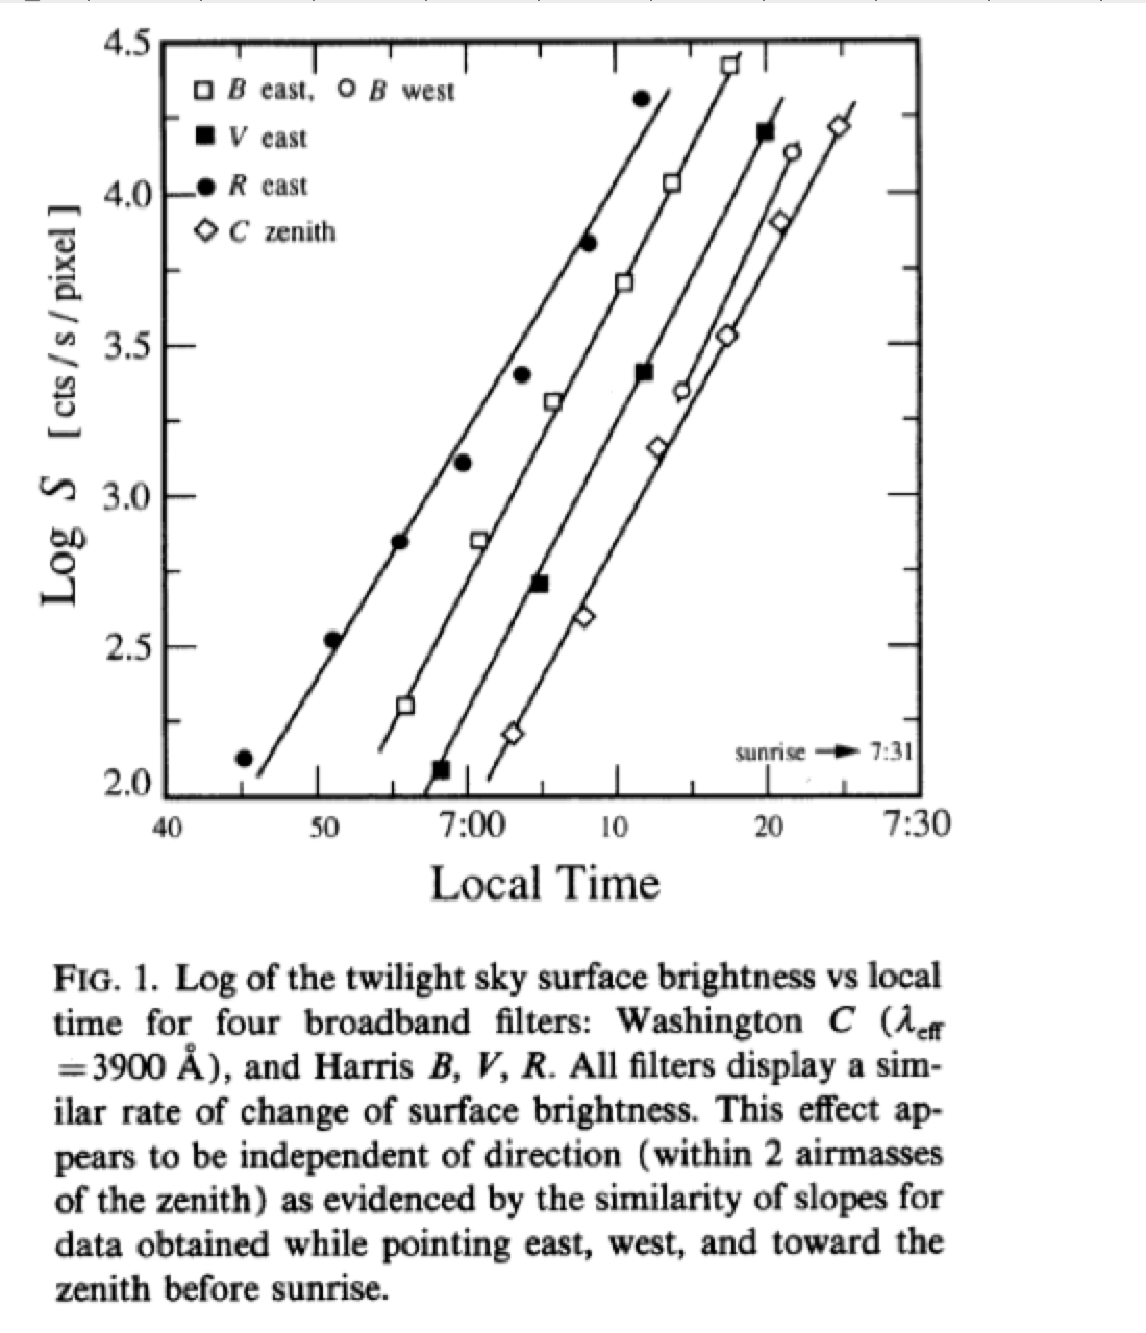
\includegraphics[width=6in]{figs/Stubbs_Fig1.pdf}
\caption{(reproduced from Tyson et al, 1993). This plot shows that the sky brightness changes by one magnitude in a 4.2 minute interval, essentially independent of passband.}
\label{default}
\end{center}
\end{figure}

Figure 2 illustrates the principles that underpin this proposal. LSST is a unique combination of hardware and software, that will deliver reliable catalogs of both the static and the dynamic sky. By pushing towards shorter integration times we can greatly expand the scientific reach of the system. 

The dynamic range in magnitudes that we can achieve for a given integration time depends on the sky background, the read noise, and the full well depth per pixel. We will adopt a typical value of 100Ke for the full well depth, but the arguments presented below are essentially independent of this value. The dynamic range in magnitudes is limited on the bright end by the point source whose PSF peak exceeds full well, and on the faint end by the 5$\sigma$ point source sensitivity, which depends on sky brightness per pixel. So we are squeezed between the two parameters of full well depth and sky background. 

\begin{figure}[htbp]
\begin{center}
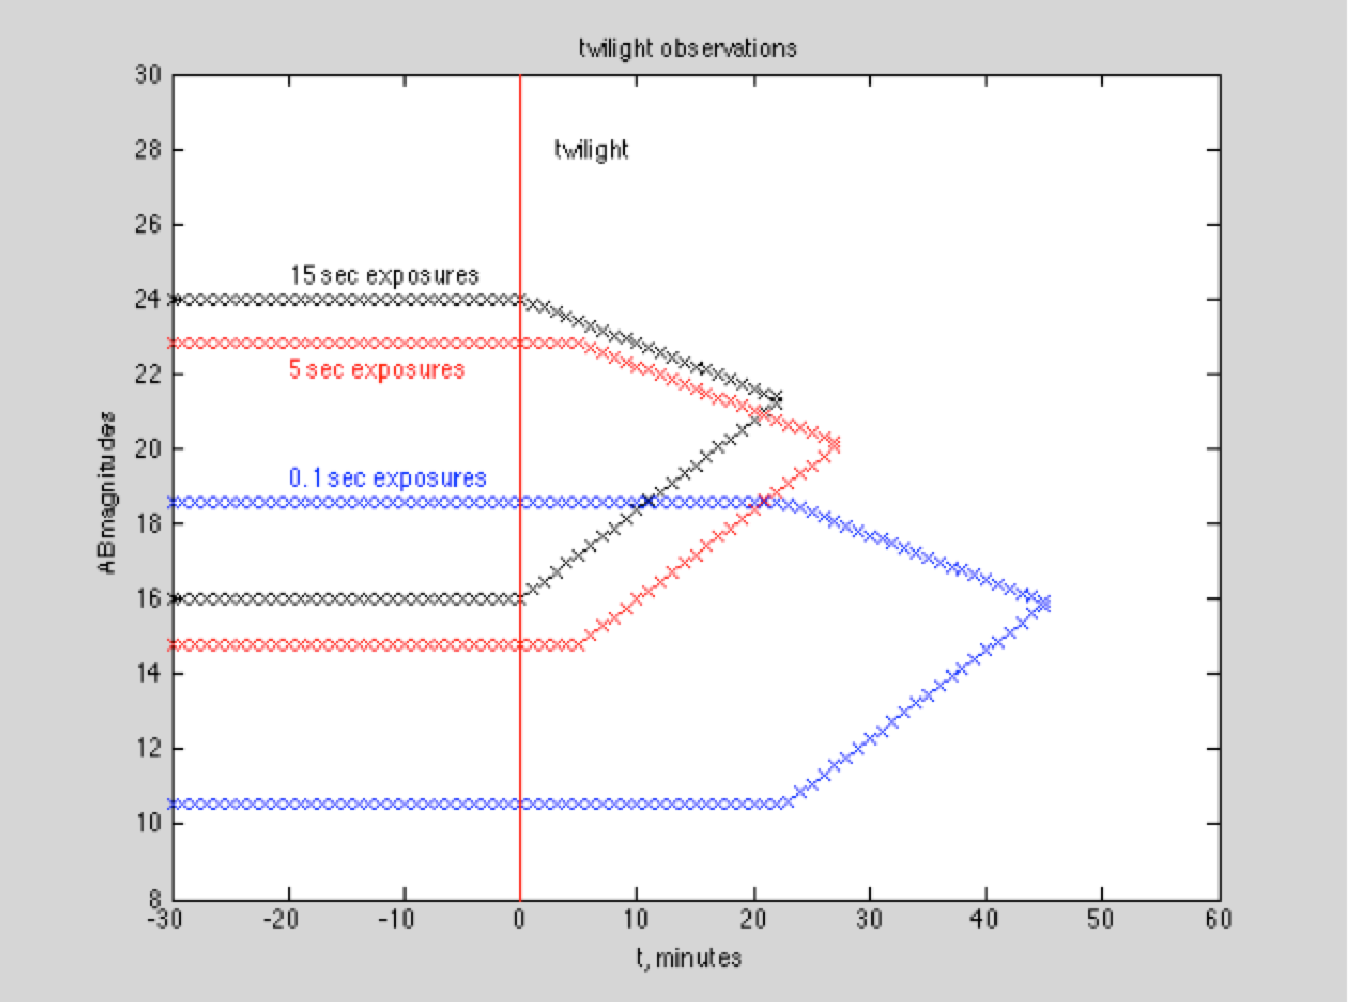
\includegraphics[width=6in]{figs/Stubbs_Fig2.pdf}
\caption{Twilight dynamic range. As we enter morning twilight time, the increasing sky brightness requires brighter sources for 5 sigma detection, and also limits unsaturated objects to increasingly fainter sources. Eventually the gap between these goes to zero. But operating at shorter exposure times allows us to push useful survey operations into brighter twilight time, and also to increase the dynamic range of the LSST survey products. The black lines correspond to 15 second integrations (nominally in the r band), the red lines to 5 second exposures, and the blue curves to 0.1 second exposures. The upper lines in each case represent the 5 sigma point source detection threshold while the lower line corresponds to the source brightness that produces saturation in the peak pixel of the PSF. Adding shorter exposure times increases our dynamic range in flux, and adds valuable observing time.}
\label{default}
\end{center}
\end{figure}

The 5 sigma limiting flux scales as the square root of the sky brightness, while the saturation flux decreases linearly as sky brightness increases. So the two curves in Figure 2 have slopes that differ by a factor of two. Operating during bright-sky time with short exposures adds about 20 minutes of observing per twilight, or 40 minutes per night. This is a non-trivial resource!

Figure 2 shows one reason why it is not advantageous to go below 0.1 second exposures- we would lose the overlap between a twilight survey and the standard LSST object catalog. 

Having set the stage for the opportunity to operate at shorter exposure times either during dark sky time, or during twilight, or both, we now describe some of the scientific motivations for doing so. 

\subsection{Science Drivers for Shorter Exposures}

\subsubsection{Discovery space at short time scales.} 

LSST is a time domain discovery machine. It is hard to anticipate the importance of being able to detect astronomical variability on short time scales. By extending the time domain sensitivity to phenomena with a characteristic time of less than 5 seconds, we will have added 1.5 orders of magnitude in time domain sensitivity. 

Taking short exposures does not necessarily imply a requirement on fast image cadence. Periodic variability can be readily detected and characterized with a succession of short images that do not satisfy the Nyquist criterion, as long as we know the time associated with each data point to adequate accuracy. But it does seem appropriate to investigate the maximum possible rapid-fire imaging rate for LSST, presumably limited by either data transfer bottlenecks or by thermal issues within the camera. 

\subsubsection{Distances to Nearby SN Ia- an essential ingredient in using supernovae to probe dark energy.}

The determination of the equation of state parameter of the Dark Energy using type Ia supernovae entails measuring the redshift dependence of the luminosity distances to objects over a range of redshifts. The low end of this redshift range is limited by peculiar velocities to considering supernovae at redshifts z$>$0.01. At this distance (distance modulus of 
$\mu$ =33) the peak brightness of a type Ia supernova is r=15 and exceeds the expected LSST point source saturation limit. 

Moreover, the rate on the sky of these bright nearby supernovae is so low that in the standard cadence we don�t expect to obtain well-sampled multiband light curves for them. But we will discover many of them on the rise. Using twilight time with short exposures to obtain appropriate temporal and passband coverage will allow us to extend the LSST SN Hubble diagram across the entire redshift range of 0.01 to 1. 

It is vitally important that we obtain these nearby-SN light curves on the same photometric system, reduced with the same data reduction pipeline, as the distant sample. This means we really must use the LSST instrument and software in order to avoid systematic errors arising from differences in photometric systems or algorithmic issues. 

We stress that this twilight SN followup campaign can be accomplished without impacting the main survey, during the roughly 20 minutes per night of twilight that would otherwise unusable at the default exposure time. We would use the brighter twilight time to obtain pointed observations on nearby supernovae, motivated by the importance of photometric uniformity described above. 

\subsubsection{A Bright Star Survey for Galactic Science.}

We could also use the added twilight time to conduct a bright star survey, and the precise astrometry and photometry from LSST can then be used in conjunction with archived data ranging from 11th to 27th AB magnitudes. This short-exposure domain would extend the LSST dynamic range in fluxes by two orders of magnitude, towards the bright end. Moreover, obtaining precise positions, fluxes and variability at these brighter magnitudes would greatly increase the overlap with the historical archive of astronomical information, including from digitized plate data. We would be able to obtain astrometric and color information to high precision, as well time series for variability studies. 

An example of an application to Milky Way structure studies comes from RR Lyrae variable stars. With a saturation magnitude of around 16th in the standard LSST survey, RR Lyrae closer than 20 kpc will be saturated in the standard LSST images. So we will lose nearly all Galactic RR Lyrae. Extending the survey�s bright limit to 11th magnitude will allow us to collect light curves for RR Lyrae beyond $\sim$ 100 parsecs, collecting essentially all Southern hemisphere Galactic RR Lyrae.

Another application for stellar population studies is measuring the fraction of binary stars as a function of stellar type, metallicity, age and environment. By conducting a variability survey in the 11-18 magnitude range we can capitalize on temperature and metallicity data already in hand for many of these objects. 

Another application of a bright star survey would be to search for planetary transits in the magnitude range appropriate for radial velocity followup observations using 30 meter class telescopes. For high dispersion spectrographs at the 4m aperture class, most targets are currently around 8th magnitude, so we should expect 30m telescopes to attain similar radial velocity precisions for sources of magnitude  8 + 5log(30/4) = 12. By going to shorter exposures we obtain almost an hour�s additional observing time per night when these sources don�t saturate, whereas they are far beyond saturation in the default 15 second LSST survey images. 

A typical (r$-$K) color between SDSS and 2MASS is r$-$K=3. The 2MASS catalog is complete down to K$\sim$14 which corresponds to r$\sim$17. So most 2MASS stars will be saturated in the standard LSST 15 second observations. A bright star survey will allow a multiband match to the 2MASS data, as well as an astrometric comparison between the two catalogs. 

Finally, the apparent magnitude of solar system objects depends on their distance from us and from the sun, as well as illumination and observation geometry. Extending the bright limit will allow us to track asteroid positions as they approach opposition.  

\subsection{Counterarguments}

\subsubsection{What About Scintillation Effects?}

Short exposure times suffer from scintillation effects. An estimate for uncertainty due to scintillation is provided by 
\url{http://astro.corlan.net/gcx/scint.txt}. For a 0.1 second integration we expect a fractional flux uncertainty of  0.15 at 2 airmasses and 0.043 at 1 airmass, for a 10 cm aperture. Scaling this up to the 8.5m aperture of LSST by a factor D$^{2/3}$ predicts fractional flux variations of below one percent, even at two airmasses, for a 0.1 second exposure. So scintillation should not impact our ability to make precision measurements of flux and position.  

\subsubsection{What about just doing this with smaller telescopes?}

A possible counter-argument to the proposal of allowing for shorter exposure times is that much of this can be done with smaller telescopes. But it�s important to bear in mind that LSST is a system, and the data reduction and dissemination tools are as important as the hardware. We intend to deliver accessible, high-quality, well-calibrated photometry on a common photometric system and correspondingly good positions. If we do so from a co-added point source depth of 27th to the short-exposure bright limit of 11th magnitude we will span over six decades in flux on a well-calibrated flux scale. We would also have the ability to study astrophysical variability on time scales from 0.1 second to 10 years, which is nine decades in the time domain. This combination of temporal and flux dynamic range would be a truly remarkable  achievement, and would yield science benefits far beyond the illustrative examples provided above. Much of this discovery space is enabled by going to shorter exposures. 
 
\subsection{Proposed Implementation and Impacts}

The implementation of this would simply entail taking short-exposure images during twilight time that would otherwise go unused. The data rate would go up, and the number of shutter cycles per night would also increase. 
%
%\section{References}
%
%Tyson and Gal, An Exposure Guide for Taking Twilight Flats with Large Format CCDs, AJ {\bf 105}, 1026 (1003). 




% --------------------------------------------------------------------

% \input{commissioning.tex}

% --------------------------------------------------------------------

\navigationbar
